\documentclass{beamer}
\usepackage{pgfplots}
\usepackage{pgf-pie} % para o gráfico de pizza
\pgfplotsset{compat=1.17}

% Tema e cores
\usetheme{Madrid}

% Configurações
\title{Projeto: Seja um Empreendedor}
\subtitle{Matemática no Dia a Dia}
\author{1º Ano do Ensino Médio}
\date{}

\begin{document}

% CAPA
\begin{frame}
    \titlepage
\end{frame}

% APRESENTAÇÃO
\begin{frame}{O que vamos fazer?}
    Neste projeto, você e seu grupo vão criar uma \textbf{ideia de negócio simples}, usando a Matemática para:
    \begin{itemize}
        \item Definir um produto ou serviço
        \item Calcular preços, custos e lucros
        \item Fazer previsões de vendas
        \item Construir tabelas e gráficos
        \item Criar fichas e etiquetas
        \item Apresentar sua proposta de forma criativa
    \end{itemize}
\end{frame}

% EXEMPLOS DE NEGÓCIO
\begin{frame}{Exemplos de Negócios}
    Vocês podem escolher ideias simples, como:
    \begin{itemize}
        \item Venda de sucos, doces ou pipoca
        \item Chaveiros artesanais
        \item Desenhos personalizados
        \item Conserto de bicicleta
        \item Bijuterias ou lembrancinhas
    \end{itemize}
\end{frame}

% O QUE DEVE TER NO TRABALHO
\begin{frame}{O que o trabalho deve ter}
    Cada grupo precisa entregar:
    \begin{enumerate}
        \item Nome do negócio
        \item Produto ou serviço ofertado
        \item Preço de venda de cada item
        \item Cálculo de custos e lucro esperado
        \item Tabela com previsão de vendas
        \item Gráfico (colunas ou pizza) mostrando os resultados da enquete
        \item Desenho ou esquema do espaço de venda/embalagem
        \item Ficha de controle e etiquetas de preços
    \end{enumerate}
\end{frame}

% EXEMPLO DE TABELA
\begin{frame}{Exemplo de Tabela de Vendas}
    \begin{tabular}{|c|c|c|c|}
        \hline
        Produto & Custo (R\$) & Preço (R\$) & Lucro (R\$) \\
        \hline
        Suco de Laranja & 2,00 & 3,50 & 1,50 \\
        Suco de Uva     & 2,50 & 4,00 & 1,50 \\
        \hline
    \end{tabular}
\end{frame}

% EXEMPLO DE GRÁFICO DE COLUNAS
\begin{frame}{Exemplo de Gráfico de Colunas}
\centering
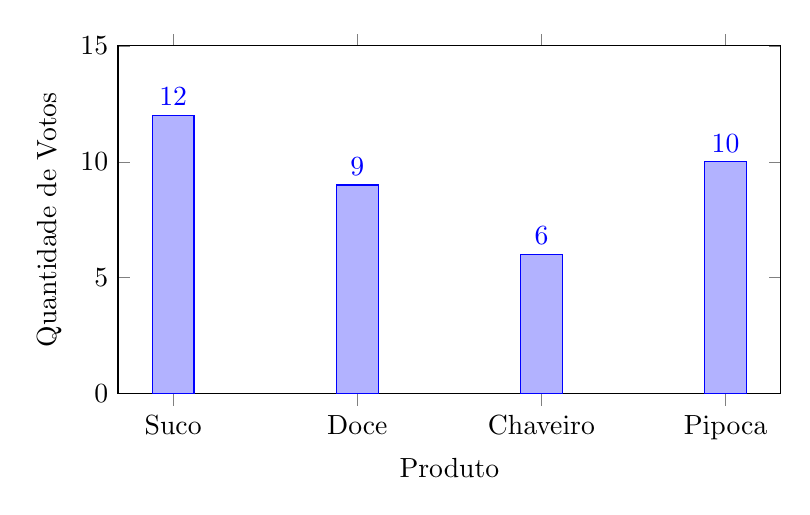
\begin{tikzpicture}
\begin{axis}[
    ybar,
    bar width=15pt,
    width=10cm,
    height=6cm,
    xlabel={Produto},
    ylabel={Quantidade de Votos},
    symbolic x coords={Suco, Doce, Chaveiro, Pipoca},
    xtick=data,
    nodes near coords,
    ymin=0,
    ymax=15
]
\addplot coordinates {(Suco,12) (Doce,9) (Chaveiro,6) (Pipoca,10)};
\end{axis}
\end{tikzpicture}
\end{frame}

% EXEMPLO DE GRÁFICO DE PIZZA
\begin{frame}{Exemplo de Gráfico de Pizza}
\centering
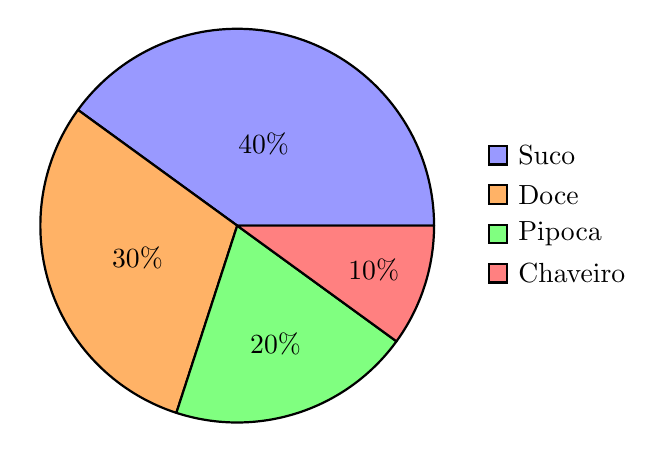
\begin{tikzpicture}
\pie[
    text=legend,
    radius=2.5,
    color={blue!40, orange!60, green!50, red!50}
]{
    40/Suco,
    30/Doce,
    20/Pipoca,
    10/Chaveiro
}
\end{tikzpicture}
\end{frame}

% FICHAS E ETIQUETAS
\begin{frame}{Fichas e Etiquetas}
    Para organizar melhor o negócio, cada grupo deve produzir:
    \begin{itemize}
        \item \textbf{Ficha de Controle:} 
        \begin{itemize}
            \item Estoque inicial
            \item Quantidade vendida
            \item Receita total
        \end{itemize}
        \item \textbf{Etiquetas de Preço:} 
        \begin{itemize}
            \item Nome do produto e valor
            \item Simples, feitas à mão ou no computador
        \end{itemize}
    \end{itemize}
\end{frame}

% EXEMPLO DE FICHA
\begin{frame}{Exemplo de Ficha de Controle}
\centering
\begin{tabular}{|c|c|c|c|}
\hline
Produto & Quantidade Inicial & Vendido & Estoque Final \\
\hline
Suco de Laranja & 20 & 15 & 5 \\
Doce Caseiro & 30 & 22 & 8 \\
Chaveiro & 15 & 10 & 5 \\
\hline
\end{tabular}
\end{frame}

% CRONOGRAMA
\begin{frame}{Passo a Passo}
    \begin{enumerate}
        \item Introdução ao projeto
        \item Estudo de medidas, proporções e sistema monetário
        \item Construção de tabelas, gráficos, fichas e etiquetas
        \item Desenvolvimento da ideia de negócio
        \item Apresentação final na feira
    \end{enumerate}
\end{frame}

% DICAS
\begin{frame}{Dicas para o Sucesso}
    \begin{itemize}
        \item Criatividade conta muito!
        \item Trabalhem juntos (cooperação é essencial).
        \item Usem a matemática como ferramenta para dar clareza à ideia.
        \item Sejam organizados e claros na apresentação.
    \end{itemize}
\end{frame}

% ENCERRAMENTO
\begin{frame}{Vamos Empreender!}
    \centering
    \Huge \textbf{Agora é com vocês!} \\
    \vspace{0.5cm}
    \Large Criem, calculem e apresentem sua ideia de negócio! 🚀
\end{frame}

\end{document}

